\documentclass[12pt,a4paper]{report}

\usepackage[utf8]{inputenc}
\usepackage[english]{babel}
\usepackage{amsmath}
\usepackage{amsfonts}
\usepackage{amssymb}
\usepackage{graphicx}
\usepackage{eurosym}
\usepackage[left=2cm,right=2cm,top=2cm,bottom=2cm]{geometry}
\usepackage{wrapfig}
\usepackage{mathdots}
\usepackage{caption}
\usepackage{cite}
\usepackage{mathrsfs}
\usepackage{float}
\usepackage{hyperref}

\author{Josep Maria Serra Moncunill}
\title{Network Layer Protocols}
\date{\today}


\begin{document}

\maketitle
\tableofcontents
\listoffigures
\listoftables

\section{Major failure deffinition}

\paragraph{}In Project Charter, it has been stated that a major failure can be defined as the loss of a client’s satellite coverage because of a failure in the network. However, this deffinition is not enough precise. For example, during a communication, it can happen that a data packet is lost, or has an error and it is discarded. This means that, for that packet, the communication was lost, but it dones not mean that the communication with the client was lost. Another aspect to take into account is that a satellite may fail, but an alternative path can still exist and, therefore, the communication can continue. Morover, if the client satellite loses all communication with all satellites in range, due to the different orbital velocities of the client satellite and the network satellites, the client satellite will eventually be in range of a functional network satellite.

\paragraph{}For all this reasons, a more specific criteria is needed. In Project Charter it has also been stated that the network will provide communication between a client satellite and a ground station with a latency lower than 5 minutes (300 seconds, or 300,0000 miliseconds). A major failure will consiste in a failure in the network that causes a message to arrive from a client satellite to a client ground station with more that 5 minutes of delay, or not arrive at all. Derived from this deffinition, a minor failure can also be deffined. It can be defined as a delay of more that 5 minutes in a communication between a client satellite and a ground station without any failure in the network.

\subsection{Major failure}

\paragraph{}Because of the different height of the client satellite and the network satellites, if all the network satellites is range of the client satellite fail, the client satellite may come in range of a working network satellite if enough time passes. In some cases, this can happen in less than 5 minutes and, therefore, it will not be considered a major failure. For this reason, a more critical situation will be considered. It will be considered that the client satellite moves at the same speed as the network satellites, in the same orbital plane. In this situation, a major failure can happen because for two reasons: all network satellites in range of the client satellite fail, or some fail but the alternative path takes more that 5 minutes to transmit the information.

\paragraph{}The first reason will be evaluation in the following lines. Depending on the location of the satellite and the distribution of the satellites in the constellation, the number of adjacent satellites may vary. A satellite over the ecuator can have up to six adjacent satellites. In this case, if a client satellite only communicates with this network satellite, a major failure will be a failure in all 6 adjacent satellites, as it can be seen in Figure \ref{fig:critical1}. However, if the client satellite has more of one network satellite in range, the number of required failures for a major failure inclreases and, if three network satellites are in range, 9 failures are required, as Figure \ref{fig:critical3} shows. In another case, if the adjacent plane move in a different direction, the number of adjacent satellites is 4 if the client satellite only can communicate with one satellite, like in Figure \ref{fig:critical1C}, or 6 if it can communicate with three, as in \ref{fig:critical3C}. As the satellites aproach the poles, the distances between each plane decreases and, therefore, the number of adjacent satellites incleases, as well as the number of satellites needed for a major failure. The number of satellites in range of the client satellite will also increase, therefore, the likelyhood of a major failure happening near the pole is small.
\begin{figure}[H]
\begin{center}
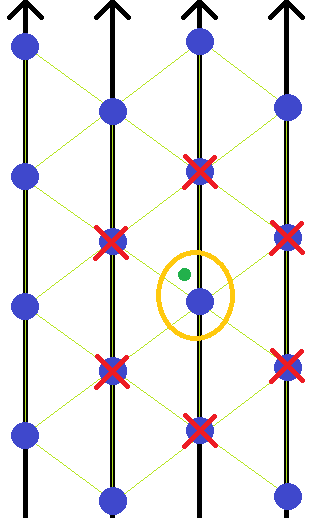
\includegraphics[scale=0.5]{critical1.PNG}
\caption[1 communication range failure]{Failure due to the loss of all possible communication satellites if the client can communicate to only one network satellite.}
\label{fig:critical1}
\end{center}
\end{figure}
\begin{figure}[H]
\begin{center}
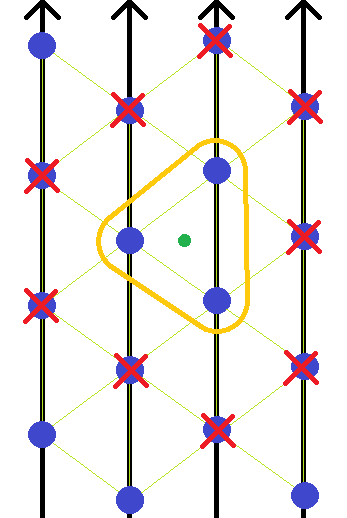
\includegraphics[scale=0.5]{critical3.PNG}
\caption[3 communication range failure]{Failure due to the loss of all possible communication satellites if the client can communicate to three network satellite.}
\label{fig:critical3}
\end{center}
\end{figure}
\begin{figure}[H]
\begin{center}
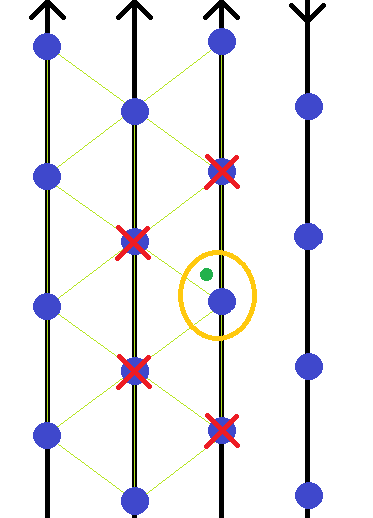
\includegraphics[scale=0.5]{critical1C.PNG}
\caption[1 communication failure counter-direction]{Failure due to the loss of all possible communication satellites if the client can communicate to only one network satellite and the adjacent plane moves in the opposite direction.}
\label{fig:critical1C}
\end{center}
\end{figure}
\begin{figure}[H]
\begin{center}
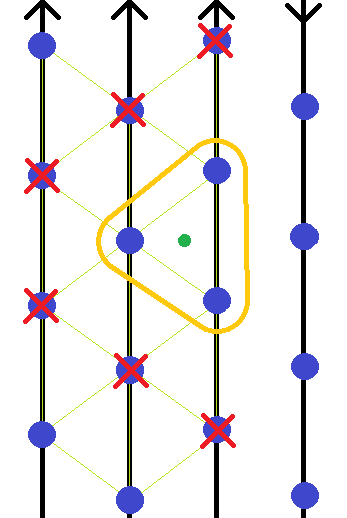
\includegraphics[scale=0.5]{critical3C.PNG}
\caption[1 communication satellite failure counter-direction]{Failure due to the loss of all possible communication satellites if the client can communicate to three network satellite and the adjacent plane moves in the opposite direction.}
\label{fig:critical3C}
\end{center}
\end{figure}

\paragraph{}In the following lines, a major failure due to a delay supperior to 5 minutes originated by a failure will be evaluated. First of all, it is needed to evaluate the transmission time. The minimmum data rate that will handle the satellites is 25 Mbit/s. Therefore, it will be considered 25 Mbit/s as the data rate of the satellites, since it is the most restrictive. The protocols chosen, by deffault, cannot handle data units of more than 62,500 bytes, aproximately. This is 500.000 bits. With the data rate chosen, the time to transmit this information is 0.02 seconds. For a path of 20 nodes, and considering that a satellites recives the entire packet before sending it again, the transmission time will be 0.4 seconds. The transmission is done using electromagnetic waves, which move at the speed of light. For this short distances, it can be considered to be instantaneously. The time used to process each data packet has to be taken into account. If each node needs 1 second to process the packet, the total processing time will be 20 seconds. Finally, the time to recognize a fallen satellite and the time to compute an alternative route is requires. By deffault, OSPF protocol requires 40 seconds of no response to label an adjacent node as dead. When this time expires, the fallen link state will be transmitted. When a node recieves this update, it will wait 5 seconds and then it will calculate new routes. If the process requires 60 seconds, the total time until a failure happens and a new route is calculated is 105 seconds. With the processing time of 20.4 seconds, two nodes can fail and the path can be recalculated two times, and the message will arrive at the ground station in less than 5 minutes.

\paragraph{}It can be concluded that a major failure can happen due to various factors. One of them is the failure of all the satellites surrounding the satellites in range of the client satellite. This can be up to 9 satellites. Another case of major failure is theconsecutive failures of satellites in the communication path. In this case, three satellites is enough to cause a major failure if each one fails when a route has been calculated.

\end{document}